% !TEX root =  ../STVR-model-seeding.tex

%%%%%%%%%%%%%%%%%%%%%%
\section{Background And Related Work}\label{sec:model_seeding:background}
%%%%%%%%%%%%%%%%%%%%%%

%\subsection{Automated crash reproduction}

Application crashes that happen while the system is operating are usually reported to developer teams through an issue tracking system for debugging purposes~\cite{DBLP:conf/iwpc/WhiteVJBP15}. Depending on the amount of information reported from the operation environment, this debugging process may take more or less time. Typically, the first step for the developer is to try to reproduce the crash in his development environment~\cite{Zeller2009}. Various approaches~\cite{Chen2015, Nayrolles2017, Xuan2015, BPT17concrash, soltani2017} automate this process and generate a \emph{crash-reproducing test case} without requiring human intervention during the generation process.  Previous studies~\cite{Chen2015,Soltani2018a} show that such test cases are helpful for the developers to debug the application.

\begin{lstlisting}[
firstnumber=0,
caption={Stack trace of the XWIKI-13372 crash},
label=lst:model_seeding:stacktrace,
float=t]
java.lang.NullPointerException: null
  at com[...]BaseProperty.equals([...]:96)
  at com[...]BaseStringProperty.equals([...]:57)
  at com[...]BaseCollection.equals([...]:614)
  at com[...]BaseObject.equals([...]:235)
  at com[...]XWikiDocument.equalsData([...]:4195)
  [...]
\end{lstlisting}

For Java programs, the information reported from the operations environment ideally includes a \emph{stack trace}. For instance, Listing \ref{lst:model_seeding:stacktrace} presents a stack trace coming from the crash XWIKI-13372.\footnote{Described in  issue \url{https://jira.xwiki.org/browse/XWIKI-13372}.} The stack trace indicates the \emph{exception} thrown (\texttt{Null\-Pointer\-Exception} here) and the \emph{frames}, \ie the stack of method calls at the time of the crash, indexed from 1 (at line 1) to 26 (not shown here).

Various approaches use a stack trace as input to automatically generate a test case reproducing the crash.
%
\textsc{CONCRASH}~\cite{BPT17concrash} focuses on reproducing \textit{concurrency} failures that violate thread-safety of a class by iteratively generating test code and looking for a thread interleaving that triggers a concurrency crash. %To drive the test generation process and avoid expensive computations, \textsc{CONCRASH} applies pruning strategies to avoid redundant and irrelevant test code.
%
\textsc{JCHARMING}~\cite{nayrolles2015jcharming,Nayrolles2017} applies model checking and program slicing to generate crash reproducing tests. %Since \textsc{JCHARMING} can be applied to any frame from a given crash stack trace, the approach can reproduce any fraction of the target crash stack trace.
%
\textsc{MuCrash}~\cite{Xuan2015} exploits existing test cases written by developers. \textsc{MuCrash} selects test cases covering classes involved in the stack trace and mutates them to reproduce the crash.
%Test cases covering the classes in the stack trace are selected and mutated to reproduce the crash.
%
\textsc{STAR} \cite{Chen2015} applies optimized backward symbolic execution to identify preconditions of a target crash and uses this information to generate a crash reproducing test that satisfies the computed preconditions.
%
Finally, \textrm{RECORE} \cite{Rossler2013} applies a search-based approach to reproduce a crash using  both a stack trace and a core dump produced by the system when the crash happened to guide the search.


\subsection{Search-Based Crash Reproduction}

Search-based approaches have been widely used to solve complex, non-linear software engineering problems, which  have multiple and sometimes conflicting optimization objectives~\cite{Harman2012}. Recently, Soltani \etal~\cite{soltani2017} proposed a search-based approach for crash reproduction called \evocrash. \evocrash is based on the \evosuite approach \cite{fraser2012whole,Fraser2014b} and applies a new \textit{guided genetic algorithm} to generate a test case that reproduces a given crash using a distance metric, similar to the one described by Rossler \etal \cite{Rossler2013}, to guide the search.
%
For a given stack trace, the user specifies a \emph{target frame} relevant to his debugging activities: \ie the line with a class belonging to his system, from which the stack trace will be reproduced. For instance, applying \evocrash to the stack trace from Listing \ref{lst:model_seeding:stacktrace} with a target frame~2 will produce a crash-reproducing test case for the class \texttt{BaseStringProperty} that produces a stack trace with the same two first frames. 

Soltani \etal~\cite{soltani2017} demonstrated the usefulness of the tests generated by \evocrash for debugging and code fixing. They also compared \evocrash to \evosuite and showed that \evocrash reproduces more crashes (85\%) than \evosuite (33\%), and, for the crashes reproduced by both approaches, \evocrash took on average 145 seconds while \evosuite took on average 391 seconds. These results illustrate the limitations of high-code-coverage-driven test case generation and the need for adequate guidance for crash reproduction. 

An overview of the \evocrash approach is shown at the right part of Figure~\ref{fig:approach} (box 5). The first step of this algorithm, called \emph{guided initialization}, is used to generate a random population. This random population is a set of random unit tests where a \emph{target method}  call (\ie the method in the target frame) is injected in each test. During the search, classical guided crossover and guided mutation are applied to the tests in such a way that they ensure that only the tests with a call to the target method are kept in the evolutionary loop.
%
The overall process is guided by a \emph{weighted sum fitness function} \cite{Soltani2018b}, applied to each  test $t$:
\begin{equation} \label{fitness_function}
%
fitness(t) = 3 \times d_{l}(t) + 2 \times d_{e}(t) + d_{s}(t)
%
\end{equation}

The terms correspond to the following conditions when executing the test:
\begin{inparaenum}[(i)]
\item whether the execution distance from the target line ($d_{l}$) is equal to $0.0$, in which case,
\item if the target exception type is thrown ($d_{e}$), in which case,
\item if all frames, from the beginning up until the selected frame, are included in the generated trace ($d_{s}$).
\end{inparaenum}
The overall fitness value for a given test case ranges from $0.0$ (crash is fully reproduced) to $6.0$ (no test was generated), depending on the conditions it satisfies.

%In this work, we implemented the \evocrash approach in our crash reproduction toolset called \botsing\footnote{Available at ...}.
%\todo{Add double-blinded URL}

\subsection{Seeding Strategies For Search-Based Testing}

In addition to guided search, a promising technique is \textit{seeding}. Seeding strategies use related knowledge to help the generation process and optimize the fitness of the population~\cite{Fraser2012, Chen2018b, Lopez-Herrejon2014a}. We focus here on the usage of the source code and the available tests as primary sources of information for search-based testing. Other approaches, for instance, search for string inputs on the internet \cite{McMinn2012}, or use the existing test corpus \cite{Toffola2017} to mine relevant formatted string values (\eg XML or SQL statements).

\subsubsection{Seeding from the source code}

Three main seeding strategies exploit the source code for search-based testing \cite{Rojas2016, Fraser2012, Alshahwan2011}:
%
\begin{inparaenum}[(i)]
\item \emph{constant seeding} uses static analysis to collect and reuse constant values appearing in the source code (\eg constant values appearing in boundary conditions);
%
\item \emph{dynamic seeding} complements constant seeding by using dynamic analysis to collect numerical and string values, observed only during the execution of the software, and reuse them for seeding; and
%
\item \emph{type seeding} is used to determine the object type that should be used as an input argument, based on a static analysis of the source code (\eg by looking at \texttt{instanceof} conditions or generic types for instance).
\end{inparaenum}

\subsubsection{Seeding from the existing tests}
\label{ssec:background:testseeding}

Rojas \etal~\cite{Rojas2016} suggest two test seeding strategies, using \emph{dynamic analysis} on existing test cases: \emph{cloning} and \emph{carving}.
Dynamic analysis uses code instrumentation to trace the different methods called during an execution, which, compared to static analysis, makes it easier to identify inter-procedural sequences of method calls (for instance, in the context of a class hierarchy). Cloning and carving have been implemented in \evosuite and can be used for unit test generation.

For cloning, the execution of an existing test case is copied and used as a member of the initial population of a search process. Specifically, after its instrumentation and execution, the test case is reconstructed internally (without the assertions), based on the execution trace of the instrumented test. This internal representation is then used as-is in the initial population. Internal representation of the cloned test cases are stored in a \emph{test pool}.

For carving, an object is reused during the initialization of the population and mutation of the individuals.
In this case, only a subset of an execution trace, containing the creation of a new object and a sequence of methods called on that object, is used to internally build an object on which the methods are called. This object and the subsequent method calls are then inserted as part of a newly created test case (initialization) or in an existing test when a new object is required (mutation). Internal representations of the carved objects\footnote{In this paper, we use the term \emph{object} to refer to a carved object, \ie an object plus the sequence of methods called on that object.} are stored in an \emph{object pool}.

The integration of seeding strategies into crash reproduction is illustrated in Figure~\ref{fig:approach}, box 5.
As shown, the test cases (respectively objects) to be used by the algorithm are stored in a test case (respectively object) pool, from which they can be used according to user-defined probabilities.
For instance, if a test case only contains the creation of a new \texttt{LinkedList} (using \texttt{new}) that is  filled using two \texttt{add} method calls, the sequence, corresponding to the execution trace $<$\texttt{new}, \texttt{add}, \texttt{add}$>$, may be used as-is in the initial population (cloning) or inserted by a mutation into other test cases (carving).

\subsubsection{Challenges in seeding strategies}

The existing seeding techniques use only one resource to collect information for seeding. However, it is possible that the selected resource does not provide enough information about class usages. For instance, test seeding only uses the carved call sequences from the execution of the existing test cases. If the existing test cases do not cover the behavior of the crash in the interesting classes, this seeding strategy may even misguide the search process. Additionally, if the number of observed call sequences is large, the seeding strategy needs a procedure to prioritize the call sequences for seeding. Using random call sequences as seeds can sometimes misguide the search process. Existing seeding strategies do not currently address these issues.

\subsection{Behavioral Model-Based Testing}

 \begin{figure}[!t]
    \centering
    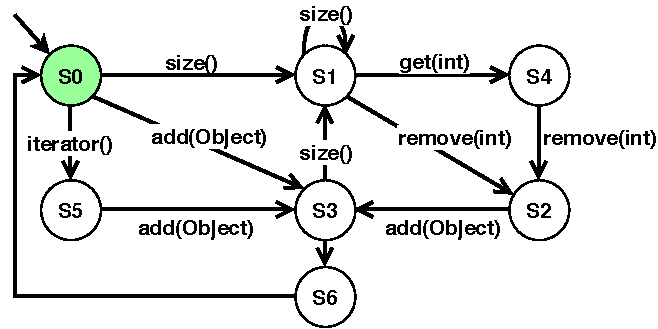
\includegraphics[width=0.55\textwidth]{papers/model_seeding/figures/list.pdf}
    \caption{Transition system for method call sequences of the class \texttt{java.util.LinkedList} derived from Apache commons math source code and test cases.}
    \label{fig:list}
\end{figure}

%Similarly to search-based testing, behavioral model-based testing seeks to select a relevant set of test cases.
\textit{Model-based testing} \cite{Utting2007} relies on abstract specifications (models) of the system under test to support the generation of relevant (abstract) test cases.  \textit{Transition systems} \cite{Baier2007} have been used as a fundamental formalism to reason about test case generation and support the definition of formal test selection criteria \cite{Tretmans2008}.
%
Each abstract test case corresponds to a sequence of method calls on one object: \ie a path in the transition system starting from the initial state and ending in the initial state, a commonly used convention to deal with finite behaviours \cite{Devroey2017b}.
Once selected from the model, abstract test cases are concretized (by mapping the transition system's paths to concrete sequences of method calls) into \emph{executable test cases} to be run on the system.
In this paper, we derive abstract test cases (called \emph{abstract object behavior} hereafter) and concretize them, producing pieces of code creating objects and invoking methods on such objects. Those pieces of code serve as seeds for search-based crash reproduction.

Figure \ref{fig:list} shows an example of a transition system representing the possible \emph{sequences} of method calls on \texttt{java.util.List} objects. Figure  \ref{fig:list} illustrates usages of methods in \texttt{java.util.List} objects, learned from the code and tests, in terms of a transition system, from which \textit{sequences} of methods calls can be derived.
%

The obtained transition system subsumes the behavior of the sequences used to learn it but also allows for new combinations of those sequences.  These behaviors are relevant in the context of seeding as the diversity of the objects induced is useful for the search process. Also, generating invalid behaviors from the new combinations is not a problem here as they are detectable during the search process.

%Derived sequences may correspond to the original sequences, but also combinations of those sequences. Hence the behavior described by the model is richer and subsumes the behavior of the sequences used to learn it. This property is very useful for seeding in search-based software testing as it allows better diversity of the objects, which helps during the search process.

%A transition system is composed of a set of states with an initial state ($s_0$ in Figure \ref{fig:list}) and transitions. Each transition may be labeled with an action, representing here a method call.


\subsubsection{Abstract object behavior selection}

The abstract object behaviors are selected from the transition system according to criteria defined by the tester. In the remainder of this paper, we use \emph{dissimilarity} as selection criteria~\cite{Cartaxo2011,Hemmati2013}.
Dissimilarity selection, which aims at maximizing the fault detection rate by increasing diversity among test cases, has been shown to be an interesting and scalable alternative to other classical selection criteria \cite{Hemmati2013, mondal2015}.
This diversity is measured using a dissimilarity distance (here, 1 - the Jaccard index \cite{Jaccard1901}) between the actions of two abstract object behaviors.

\subsubsection{Model Inference}

The model may be manually specified (and in this case will generally focus on specific aspects of the system) \cite{Utting2007}, or automatically learned from observations of the system \cite{Herbold2017, Leemans2018, Sprenkle2013, Sprenkle2011a, Tonella2014, Verwer2017}.
In the latter case, the model will be incomplete and only contain the \emph{observed behavior} of the system \cite{Tonella2012}. For instance, the sequence $<$\texttt{new}, \texttt{addAll} $>$ is valid for a \texttt{java.util.List} object but cannot be derived from the transition system in Figure \ref{fig:list} as the \texttt{addAll} method call has never been observed.
%
The observed behavior can be obtained via static analysis \cite{Fraser2011a} or dynamically \cite{Krka:2010:UDE:1810295.1810324}. Model inference may be used for visualization \cite{Leemans2018, Verwer2017}, system properties verification \cite{Lorenzoli2008a, Ghezzi2014}, or generation \cite{Herbold2017, Sprenkle2013, Sprenkle2011a, Prowell2004, Zhang2015a, Fraser2011a} and prioritization \cite{Devroey2017b, Dulz2003} of test cases.



